%!TEX root = ../dissertation.tex

\chapter{BlendMe! - The User Study}
\label{chapter:design}
%
This chapter of the document concerns the design and implementation decisions fulfilled when developing the
supporting platform of our user color study. For the sake of simplification when describing and talking about
this platform, we have called it \emph{BlendMe!}, since its purpose is to support the collecting and analysis
of data from color blendings! \par
%
We are going to state the objectives for this user study, concretely defining the questions which we want to
have answers in the end of the study; then, we will discuss how the \emph{BlendMe!} was implemented, justifying
the decisions taken in each phase of the study. To end this section, we will define evaluation criteria which
is going to be important for the data cleaning and processing phase of the research.
%
\section{Objectives}
\label{sec:impl_objectives}
%
As seen before, there is a myriad of questions about the usage of color blendings when conveying information,
which remained unanswered. However, only a set of questions is answered in our research, since it is not possible
to reach answers to all questions. Therefore, the goals which we have picked for this User Study were to
\ul{understand if color blendings can be detected by the users}, \ul{is it easier for users to estimate the pair
of colors that resulted in a particular given blend, or reciprocally, to estimate which blend will result from a
given pair of colors}, \ul{to detect if the users follow some kind of mental convention and organize the color
when conveying the answers}, and formulate possible implications of color blending usage, in Information Visualization field of research. \par
%
Additionally, it is relevant to understand which color model stands as the best to mix colors which are, from a
perceptual point of view, more similar to the users expectation. We have planned to develop this study in two
different strands: in a \textbf{Laboratory Environment}, which will allow us to calibrate and perfectly control the
entire study conditions, and in an \textbf{Online Environment}, which will allow us to disseminate our study to a
larger set of users, even without controlling the calibration of the testing environment, but that may be useful
to corroborate the laboratory results with a larger user sample. \par
%
The questions which we think define our research goals, for this study, are:
%
\begin{itemize}
	\item \textbf{Q1:} Which Color Model best meets the users' expectations, when blending two colors?
	\item \textbf{Q2:} Do users specify the Blending-basis following some order, when users are indicating possible color
	mixtures' results?
	\item \textbf{Q3:} Are there evidences from differences across demographic groups, such as the age or gender?
\end{itemize}
%
Along the result analysis, each question will meet its answers. These questions will be explored in multiple
threads, such as:
%
\begin{enumerate*}
		\item \textbf{Analyzing the distances of each answer pair to the ideal answers of each color model}, verifying
		which color models had the best and the worst values yielded by the descriptive statistic analysis,
		\item \textbf{Evaluate the results from blendings when the basis is given to the user, against when the result
		of the blending is given},
		\item \textbf{Verify if the color models which have the best and worst results are subtractive or addictive},
		\item \textbf{Analyze the ease of blending colors}, or if
		\item \textbf{There is substantially different results among genders, or different age groups}.
\end{enumerate*}
\\ \\
%
To meet these study requirements, we drafted our study into four different phases: a \textbf{User Profiling Phase},
a \textbf{Calibration Phase}, a \textbf{Color Deficiency Test Phase} and finally, the \textbf{Core Phase}. In the
following section, we detail each of these study phases. \par
%
\section{Designing the \emph{BlendMe!}}
\label{sec:impl_designingsolution}
%
Since we aim to \emph{study to what extent can color blending techniques be used to efficiently and effectively
convey information}, it is important learn from previous results, testing out not only the validity of them but also
some missed opportunities. \par
%
One of the points discussed in section \ref{sec:background_discussion} was the amount of users who performed the study
of Gama and Gonçalves \cite{Gama20141,Gama20142}: it was large enough for their questions. However, considering the
results we aim to achieve with this study, a considerably larger sample of users is the ideal: besides conducting
the study in a laboratory environment, it is mandatory to expand the sample size by performing user studies with
online users, taking advantage of the cultural diversity that may arise. \par
%
Therefore, we intended to develop a user study which could support the laboratory controlled environment, while at
the same time supporting the collection of metrics and data from the online users: this is an important consideration,
since the workload when analyzing the results would be dramatically reduced because the data is condensed and gathered
in the same fashion, and data would be more comparable. As referred, the user study was divided onto four different
stages: the \textbf{user profiling},
\textbf{calibration testing}, \textbf{color deficiency testing} and, finally, the \textbf{principal part of the study}
where the core information was collected from the users. Each of these phases will be addressed later in this section. \par
%
When brainstorming the ideas for this study, we started with the intention of testing both the blending of two colors and
three colors; we decided that the colors which would be blended were Red (\textbf{R}), Green (\textbf{G}),
Blue (\textbf{B}), Cyan (\textbf{C}), Magenta (\textbf{M}) and Yellow (\textbf{Y}), since they represent each primitive
of the most commonly known Color Models, \ul{RGB (Additive Color Model)} and \ul{CMYK (Subtractive Color Model)}. \par
%
The color models we intended to study: the color models were \textbf{HSV, RGB, CMYK, CIE-L*a*b*} and \textbf{CIE-L*C*h*}.
These color models were picked according to previous studies conducted by Gama and Gonçalves, which have concluded that HSV
and CIE-L*C*h* were the models which generated better results \cite{Gama20141,Gama20142}; the RGB and CMYK were obvious
additions, since they are represented by their primitives and we wanted to compare the users' expectations with two
representative different color model types (additive and subtractive). Lastly, the inclusion of CIE-L*a*b* was due to the fact
that it is the color model which represents the entire range of human perceivable colors. \par
%
Then, we produced a wide spreadsheet of possible blendings of these colors, according to these color models, \textbf{mixed in
pairs of two colors} and \textbf{triples of three colors, without opposed colors in HSV angle}: this last restriction derives
from the fact that, since the HSV Color Model provides angular values for hues, there are colors from the set we have chosen
that have opposed angles (R-C, G-M and B-Y); therefore, when interpolating the angular values for these colors, the resulting color
could be obtained on another two opposed resulting angles. If we had added these color pairs to blendings with three colors,
color blendings with one of these three pairs would provide, at least, two possible outputs. Then, we have only produced blendings
of three colors which did not contain any of these three pairs, in order to simplify its future analysis. \par
%
This generated the total amount of 183 Color Blendings, being 78 from blendings of two colors and 105 from blendings of three colors. \textbf{There are 15
possible mixtures of two colors}, when combining the previous defined colors: R-G, R-B, G-B, R-C, R-M, R-Y, C-M, M-Y, G-C, G-M,
G-Y, B-C, B-M, B-Y and C-Y; on the other hand, there are 21 possible color mixtures of three colors without opposed colors in the
HSV hue circle: R-G-B, R-B-G, B-G-R, R-M-B, R-B-M, B-M-R, C-G-B, C-B-G, B-G-C, C-M-Y, C-Y-M, Y-M-C, C-M-B, C-B-M, B-M-C, C-G-Y,
C-Y-G, Y-G-C, R-M-Y, R-Y-M and Y-M-R. Figure \ref{fig:table_blends} shows an excerpt of the table produced: it depicts the results,
for each color pair, blended according to the five color models chosen.
%
\begin{figure}[htbp]
	\centering
  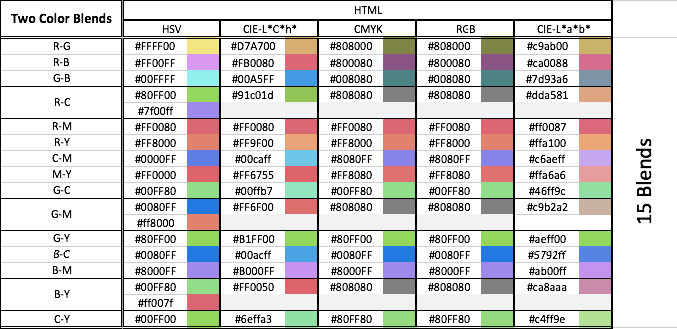
\includegraphics[width=0.8\textwidth]{images/implementation/table_blends.png}
  \caption[Excerpt of Table containing the pre-calculated Color Blends.]{Excerpt of Table containing the pre-calculated Color Blends.}
  \label{fig:table_blends}
\end{figure} \par
%
For the sake of simplicity, we have decided to drop the idea of testing the blendings of three colors, since the blendings of two
colors already produce a generous amount of possible questions, and Gama and Gonçalves already concluded that blendings of three
colors do not provide satisfactory results \cite{Gama20141}. This table was converted to \gls{CSV} file, which will be useful
in the \ul{Core Phase of the study}, which will be explained later. \par
%
\begin{table}[htbp]
	\centering
  \resizebox{0.6\textwidth}{!} {
	\begin{tabular}{cc|ccc}
		\hline
		                              & Given the Result, Asked for Basis                       &                               & \multicolumn{2}{c}{Given the Basis, Asked for Result}                                                                                                       \\ \cline{2-2} \cline{4-5}
		\multirow{-2}{*}{Question ID} & Given Color                                             & \multirow{-2}{*}{Question ID} & \multicolumn{2}{c}{Given Colors}                                                                                                                            \\ \hline
		\multicolumn{1}{c|}{1}        & \cellcolor[HTML]{FFFF00}\#FFFF00                        & \multicolumn{1}{c|}{18}       & \multicolumn{1}{c|}{\cellcolor[HTML]{FF0000}{\color[HTML]{FFFFFF} \#FF0000}} & \multicolumn{1}{c|}{\cellcolor[HTML]{00FF00}\#00FF00}                        \\ \hline
		\multicolumn{1}{c|}{2}        & \cellcolor[HTML]{FF00FF}\#FF00FF                        & \multicolumn{1}{c|}{19}       & \multicolumn{1}{c|}{\cellcolor[HTML]{FF0000}{\color[HTML]{FFFFFF} \#FF0000}} & \multicolumn{1}{c|}{\cellcolor[HTML]{0000FF}{\color[HTML]{FFFFFF} \#0000FF}} \\ \hline
		\multicolumn{1}{c|}{3}        & \cellcolor[HTML]{80FF00}\#80FF00                        & \multicolumn{1}{c|}{20}       & \multicolumn{1}{c|}{\cellcolor[HTML]{00FF00}\#00FF00}                        & \multicolumn{1}{c|}{\cellcolor[HTML]{0000FF}{\color[HTML]{FFFFFF} \#0000FF}} \\ \hline
		\multicolumn{1}{c|}{4}        & \cellcolor[HTML]{7F00FF}{\color[HTML]{FFFFFF} \#7F00FF} & \multicolumn{1}{c|}{21}       & \multicolumn{1}{c|}{\cellcolor[HTML]{FF0000}{\color[HTML]{FFFFFF} \#FF0000}} & \multicolumn{1}{c|}{\cellcolor[HTML]{00FFFF}\#00FFFF}                        \\ \hline
		\multicolumn{1}{c|}{5}        & \cellcolor[HTML]{FF0080}{\color[HTML]{FFFFFF} \#FF0080} & \multicolumn{1}{c|}{22}       & \multicolumn{1}{c|}{\cellcolor[HTML]{FF0000}{\color[HTML]{FFFFFF} \#FF0000}} & \multicolumn{1}{c|}{\cellcolor[HTML]{FF00FF}\#FF00FF}                        \\ \hline
		\multicolumn{1}{c|}{6}        & \cellcolor[HTML]{FF8000}\#FF8000                        & \multicolumn{1}{c|}{23}       & \multicolumn{1}{c|}{\cellcolor[HTML]{FF0000}{\color[HTML]{FFFFFF} \#FF0000}} & \multicolumn{1}{c|}{\cellcolor[HTML]{FFFF00}\#FFFF00}                        \\ \hline
		\multicolumn{1}{c|}{7}        & \cellcolor[HTML]{0000FF}{\color[HTML]{FFFFFF} \#0000FF} & \multicolumn{1}{c|}{24}       & \multicolumn{1}{c|}{\cellcolor[HTML]{00FFFF}\#00FFFF}                        & \multicolumn{1}{c|}{\cellcolor[HTML]{FF00FF}\#FF00FF}                        \\ \hline
		\multicolumn{1}{c|}{8}        & \cellcolor[HTML]{FF0000}{\color[HTML]{FFFFFF} \#FF0000} & \multicolumn{1}{c|}{25}       & \multicolumn{1}{c|}{\cellcolor[HTML]{FF00FF}\#FF00FF}                        & \multicolumn{1}{c|}{\cellcolor[HTML]{FFFF00}\#FFFF00}                        \\ \hline
		\multicolumn{1}{c|}{9}        & \cellcolor[HTML]{00FF80}\#00FF80                        & \multicolumn{1}{c|}{26}       & \multicolumn{1}{c|}{\cellcolor[HTML]{00FF00}\#00FF00}                        & \multicolumn{1}{c|}{\cellcolor[HTML]{00FFFF}\#00FFFF}                        \\ \hline
		\multicolumn{1}{c|}{10}       & \cellcolor[HTML]{0080FF}{\color[HTML]{FFFFFF} \#0080FF} & \multicolumn{1}{c|}{27}       & \multicolumn{1}{c|}{\cellcolor[HTML]{00FF00}\#00FF00}                        & \multicolumn{1}{c|}{\cellcolor[HTML]{FF00FF}\#FF00FF}                        \\ \hline
		\multicolumn{1}{c|}{11}       & \cellcolor[HTML]{FF8000}\#FF8000                        & \multicolumn{1}{c|}{28}       & \multicolumn{1}{c|}{\cellcolor[HTML]{00FF00}\#00FF00}                        & \multicolumn{1}{c|}{\cellcolor[HTML]{FFFF00}\#FFFF00}                        \\ \hline
		\multicolumn{1}{c|}{12}       & \cellcolor[HTML]{80FF00}\#80FF00                        & \multicolumn{1}{c|}{29}       & \multicolumn{1}{c|}{\cellcolor[HTML]{0000FF}{\color[HTML]{FFFFFF} \#0000FF}} & \multicolumn{1}{c|}{\cellcolor[HTML]{00FFFF}\#00FFFF}                        \\ \hline
		\multicolumn{1}{c|}{13}       & \cellcolor[HTML]{0080FF}{\color[HTML]{FFFFFF} \#0080FF} & \multicolumn{1}{c|}{30}       & \multicolumn{1}{c|}{\cellcolor[HTML]{0000FF}{\color[HTML]{FFFFFF} \#0000FF}} & \multicolumn{1}{c|}{\cellcolor[HTML]{FF00FF}\#FF00FF}                        \\ \hline
		\multicolumn{1}{c|}{14}       & \cellcolor[HTML]{8000FF}{\color[HTML]{FFFFFF} \#8000FF} & \multicolumn{1}{c|}{31}       & \multicolumn{1}{c|}{\cellcolor[HTML]{0000FF}{\color[HTML]{FFFFFF} \#0000FF}} & \multicolumn{1}{c|}{\cellcolor[HTML]{FFFF00}\#FFFF00}                        \\ \hline
		\multicolumn{1}{c|}{15}       & \cellcolor[HTML]{00FF80}\#00FF80                        & \multicolumn{1}{c|}{32}       & \multicolumn{1}{c|}{\cellcolor[HTML]{00FFFF}\#00FFFF}                        & \multicolumn{1}{c|}{\cellcolor[HTML]{FFFF00}\#FFFF00}                        \\ \hline
		\multicolumn{1}{c|}{16}       & \cellcolor[HTML]{FF007F}\#FF007F                        & \multicolumn{3}{c}{}                                                                                                                                                                        \\ \cline{1-2}
		\multicolumn{1}{c|}{17}       & \cellcolor[HTML]{00FF00}\#00FF00                        & \multicolumn{3}{c}{\multirow{-2}{*}{}}                                                                                                                                                      \\ \cline{1-2}
	\end{tabular}}
  \caption[Two types of questions asked about Color Blendings.]{Two types of questions asked about Color Blendings.}
  \label{table:color_blendings}
\end{table}
%
Since we wanted to \textbf{test if it is better to give the result already mixed, or indicate the blending-basis and the users create
the color mixture}, we developed a set of 32 questions to present to the user: 17 of them are of the type \textbf{presenting the resulting
color, and ask for the blending-basis}, and 15 of them are of type \textbf{given the blending-basis, ask for the blending-result}. The entire
set of questions is mapped in Table \ref{table:color_blendings}. Concerning the \ul{questions from 1 to 17}, we present the results of blending the aforementioned colors according to the HSV Color Model:
\ul{there is no concept of wrong or right answers}, but instead a referenced answer-pair for each blending result. Thus, we can compare the answer
pair given by the users with each reference pair, measuring the euclidean distance between each pair. For example, when presenting Question 1 to users,
we show a \textbf{Yellow color and expect that the answer-pair given by them is composed of Red and Green}; then, the answer-pair is interpolated in each
color model and the result is compared with the one according to each color model. Regarding \ul{questions from 18 to 32}, they present each reference-pair
(composed of two color primitives) and the users are expected to indicate a result, from the entire set of possible results depicted in Figure
\ref{fig:table_blends}. \par
%
There is a particularity among these questions: questions 2 and 3 present two different colors (\#FF00FF - \#80FF00) but, in fact, they will be compared with
the same reference pair. This is the result of blending to opposite colors (Red-Blue) which, as referred before, results into two possible results; by
presenting both results, we intend to understand to which color the users tend to. This particularity occurs with questions 10 and 11, and 15 and 16
(\#0080FF - \#FF8000, \#00FF80 - \#FF007F, respectively), which will be compared with reference pairs Green-Magenta and Blue-Yellow, correspondingly. \par
%
This user study was entirely developed used web-development libraries (\emph{e.g.} Bootstrap), technologies (\emph{e.g.} HTML5, Javascript
and CSS) and relational databases (PostgreSQL): the users are uniquely identified by a \ul{primary key (PK)} which corresponds to its user ID generated
by \emph{uniqid()} function from PHP, based on the user's timestamp, that every table from the database uses to unequivocally identify it.
An entity-relationship model maps all the information related to a given a user which will be stored for further analysis; this ER Model is present on
Figure \ref{fig:er_model}. \par
%
Being this an online published user study and known that we wanted to converge the inputs from all users in the same platform, we have executed this study
in a web browser: we have executed the majority of tests using Google Chrome and a few using Safari.
%
\begin{figure}[htbp]
	\centering
  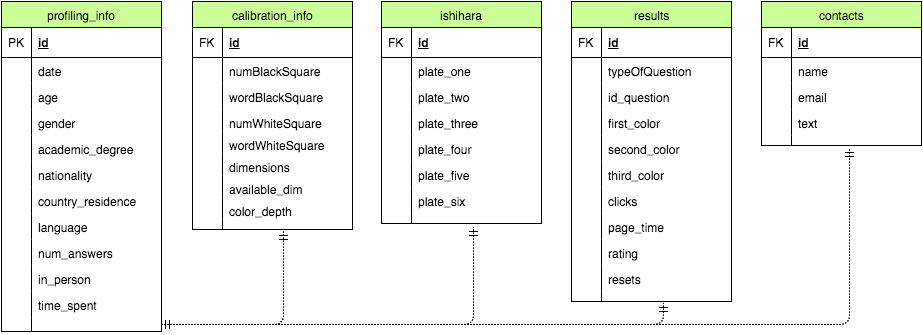
\includegraphics[width=0.8\textwidth]{images/implementation/tables_schema.png}
  \caption[Entity-Relationship Model representing the User Study information.]{Entity-Relationship Model representing the User Study information.}
  \label{fig:er_model}
\end{figure}
%
%%%%%%%%%%%%%%%%%%%%%%%%%%%%%%%%% PROFILING %%%%%%%%%%%%%%%%%%%%%%%%%%%%%%%%%%%%%%%%%%%%%%%%%%%
%
\subsection{User Profiling Phase}
\label{subsec:design_profiling}
%
In the \textbf{Profiling Phase}, questions were asked about the Age, Gender, Academic Degree, Nationality and Country of Residence: these
questions helped us conceiving user profiles with key indicators about cultural background and gender relation to results of each test.
%
We have drafted a wireframe version of this test phase, which is present in Figure \ref{fig:mockup_profiling}. This is a straight-forward
phase, in which the users are asked to indicate some demographic information. All of these information are stored in a relational database's
table called \emph{calibration\_info}, which will be entry point of the database. We had to include the \ul{Other} gender type, since it was
mandatory by Reddit to publish it online. The nationalities, academic degrees, countries of residence and native languages were all standard
JSON files which contained each set of options. \par
%
\begin{figure}[htbp]
  \centering
  \begin{minipage}{0.48\textwidth}
		\centering
	  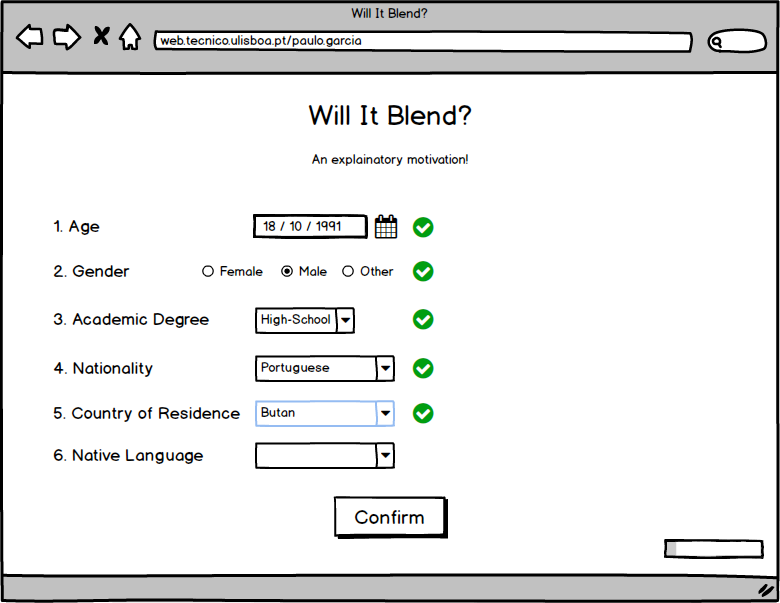
\includegraphics[width=\textwidth]{images/implementation/mockup_profiling.png}
	  \caption[Mock-up of Color Study's User Profiling Phase.]{Mock-up of Color Study's User Profiling Phase.}
	  \label{fig:mockup_profiling}
  \end{minipage}\hfill
  \begin{minipage}{0.48\textwidth}
		\centering
	  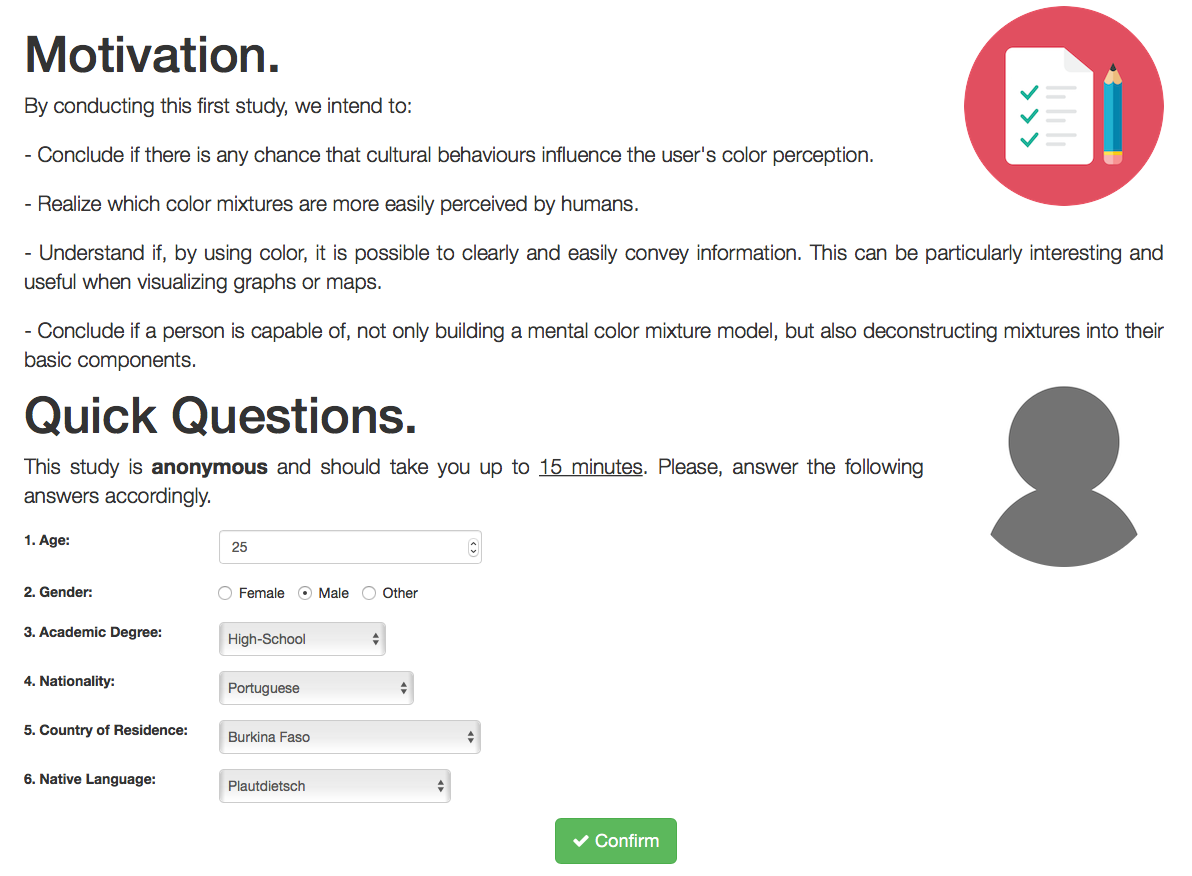
\includegraphics[width=\textwidth]{images/implementation/screen_profiling.png}
	  \caption[Screenshot of Color Study's User Profiling Phase.]{Screenshot of Color Study's USer Profiling Phase.}
	  \label{fig:screen_profiling}
  \end{minipage}
\end{figure}
%
Figure \ref{fig:screen_profiling} presents a snipping of the interface implemented for this user
study phase: be aware that this screenshot has been shrunk down to a proper scale for this document, so the proportions of the interface
are \ul{not} the ones presented to the user. \par
%
When this phase was concluded, the user was guided to another stage of the study, to perform the \textbf{Calibration Phase}, where
he was asked to analyze a set of images and answer a pair of questions. \par
%
%%%%%%%%%%%%%%%%%%%%%%%%%%%%%%%%% CALIBRATION %%%%%%%%%%%%%%%%%%%%%%%%%%%%%%%%%%%%%%%%%%%%%%%%%%%
%
\subsection{Testing Calibration Phase}
\label{subsec:design_calibration}
%
Performing online tests - specially when trying to obtain precise values about color - carries obvious problems of how it is guaranteed that
the results which may appear are, in fact, compliant with certain patterns of quality, specially color and monitor calibration patterns; to
overcome this problem, the ideal solution would be to develop a system capable of acquiring information about the user's monitor calibration,
\emph{e.g.} Brightness, Contrast, RGB Color Balance, Gamma or Saturation, as a pre-step of the study and apply an appropriate calibration when
rendering the study's main page. \par
%
\begin{figure}[htbp]
  \centering
  \begin{minipage}{0.48\textwidth}
		\centering
	  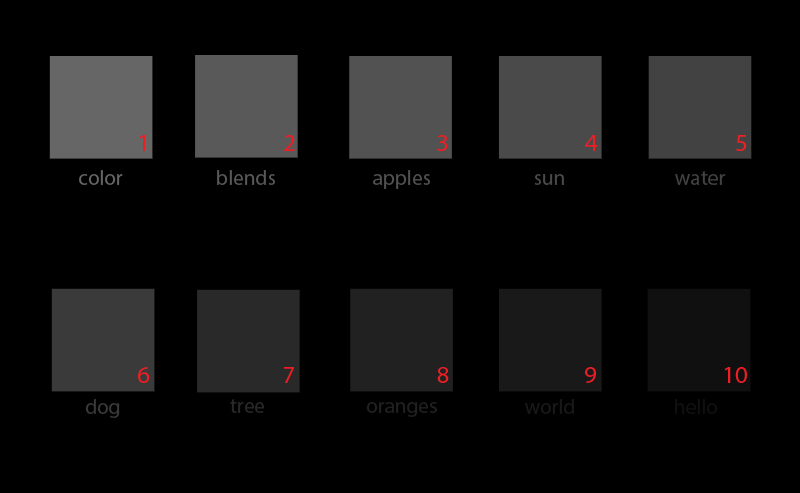
\includegraphics[width=\textwidth]{images/implementation/calibration_blackLevel.jpg}
	  \caption[Calibration image: Black-Level Measure.]{Calibration image: Black-Level Measure.}
	  \label{fig:black_level}
  \end{minipage}\hfill
  \begin{minipage}{0.48\textwidth}
		\centering
	  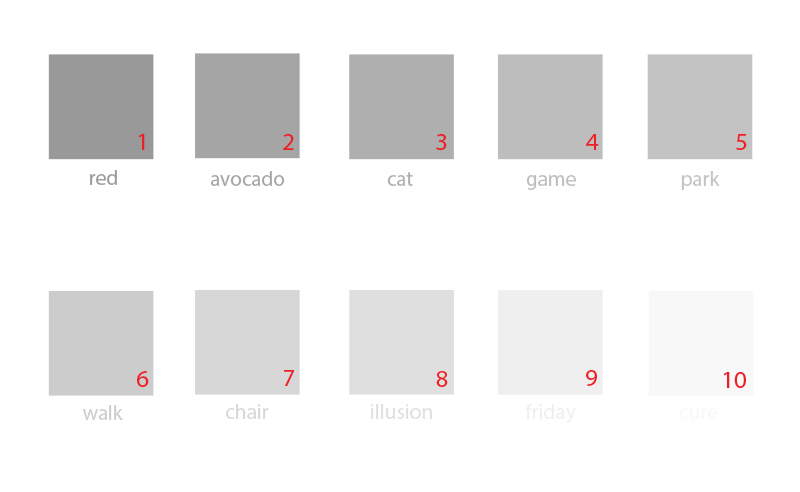
\includegraphics[width=\textwidth]{images/implementation/calibration_whiteLevel.jpg}
	  \caption[Calibration image: White-Level Measure.]{Calibration image: White-Level Measure.}
	  \label{fig:white_level}
  \end{minipage}
\end{figure}
%
Since we have not found a way to tackle this solution so far, we developed another solution for remote controlling the calibration on the
\ul{online environment}: to present two similar calibration images, one presenting a set of shaded squares ranging from grey to black shades against
a black background, and another presenting instead white squares against a white background. All of the squares presented a \ul{red number in its
corner and it was accompanied by a random word}, shaded in same color as the square it follows: the user's task was to provide us the number (and
word) from the last square which he could easily see. This information provide us input about the white-level and black-level of the screen, which
are nothing more than the \textbf{Contrast} and \textbf{Brightness}, respectively, of the display. This test is \ul{inspired in PLUGE} (stands for \textbf{P}icture
\textbf{L}ine-\textbf{U}p \textbf{G}eneration \textbf{E}quipment) Patterns, which present consecutive bars shaded between black and white, used to calibrate the black-level from a video
monitor. These calibrations images were created by us, using Adobe's Photoshop, and are presented in Figures \ref{fig:black_level} and
\ref{fig:white_level}. In the end, we have to analyze the answers to verify if they are compliant with a certain pattern of calibration acceptability,
determining if the answers of a certain user can be considered true and not misleading. \par
%
Regarding the \ul{laboratory environment}, we conducted the users tests in a LCD monitor, under a fixed light source; the monitor was calibrated
using a Spyder\footnote{"Spyder - Datacolor Imaging Solutions", Available at: \url{http://spyder.datacolor.com}. Last accessed on October 17th, 2016.}
Colorimeter which will consider the existing light in the environment and adjust the color of each pixel to a standard. This colorimeter will produce an
\emph{.icc} \textbf{color profile which will be important for the Core Test Phase}. \par
%
We have also included in this interface the \ul{protocol} to be followed when calibrating the screen, which is covered in Section \ref{sec:results_protocol}.
Figures \ref{fig:mockup_calibration} and \ref{fig:screen_calibration} represent the wireframe version of the screen, which only contained one image as
example, and the final version which was presented; however, the second one only shows the part where it was tested the black-level, since the interface
for this phase is quite extensive. \par
%
\begin{figure}[htbp]
  \centering
  \begin{minipage}{0.49\textwidth}
		\centering
	  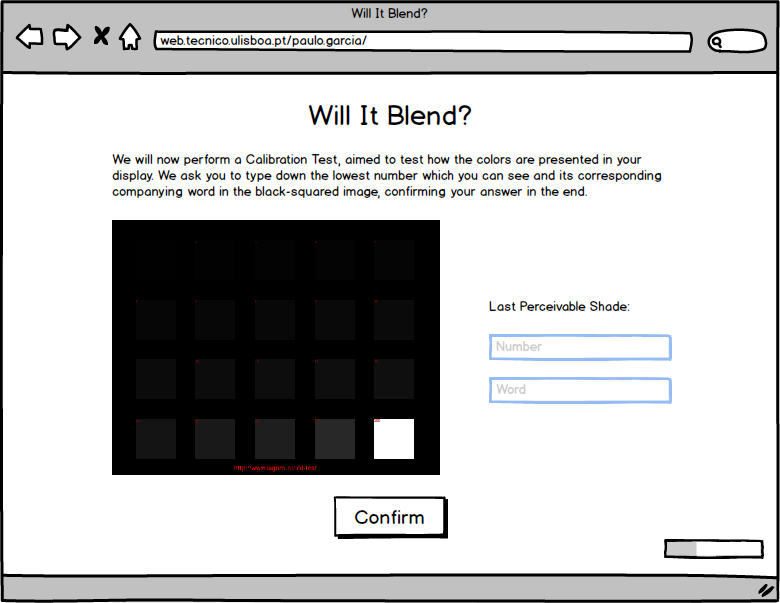
\includegraphics[width=\textwidth]{images/implementation/mockup_calibration.png}
	  \caption[Mock-up of Color Study's Calibration Testing Phase.]{Mock-up of Color Study's Calibration Testing Phase.}
	  \label{fig:mockup_calibration}
  \end{minipage} \hfill
	\begin{minipage}{0.49\textwidth}
		\centering
		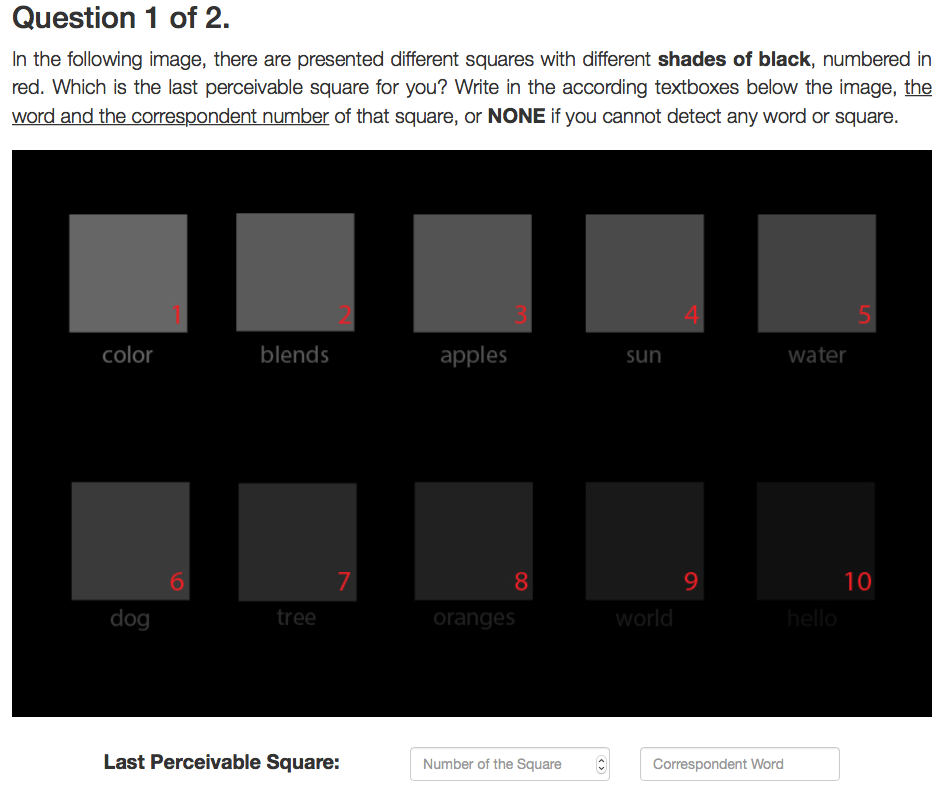
\includegraphics[width=\textwidth]{images/implementation/screen_calibration.png}
		\caption[Screenshot of Color Study's Calibration Testing Phase.]{Screenshot of Color Study's Calibration Testing Phase.}
		\label{fig:screen_calibration}
	\end{minipage}
\end{figure}
%
When this phase was concluded, the users were guided to another stage of the study, to perform the \textbf{Color Deficiency Test Phase}, where
they were asked to analyze a set colored plates and answer with its number. \par
%
%%%%%%%%%%%%%%%%%%%%%%%%%%%%%%%%% ISHIHARA %%%%%%%%%%%%%%%%%%%%%%%%%%%%%%%%%%%%%%%%%%%%%%%%%%%
%
\subsection{Testing Color Vision Deficiencies Phase}
\label{subsec:design_ishihara}
%
The Color Deficiency Test was comprised of a set of six plates, which were able to detect which type of color vision deficiencies the user
would eventually have. They could be interpreted in different ways, depending on Deficiency: this color deficiency test in commonly known as the
\emph{Ishihara Test}, which has a validated \cite{Alwis1992} short form that rearranges the order in which the plates are presented. We have only chosen plates
which detect color vision deficiencies in the Red-Green field, since it is the most common deficiency. This test was explored
in the Theoretical Background (Section \ref{subsubsec:visual_deficiencies}) of this Master Thesis. We have chosen the following plates:
%
\begin{itemize}
	\item \ul{Plate \#1} - We have chosen \cite{Alwis1992} the plate ($ID = 1$) which presents the number \textbf{12}. This is an \ul{Instruction and
	Demonstration} plate, since every user should be capable of viewing the same number and it is intended to demonstrate how to interpret the plate numbers.
	\item \ul{Plate \#2} - This plate ($ID = 4$) presents the number \textbf{29}. This a plate from the \ul{Transformation} group, presenting the number
	\textbf{29} for regular	users which do not have any color vision deficiency, and the number \textbf{70} to users which have \ul{a color vision
	deficiency in the Red-Green field}.
	\item \ul{Plate \#3} - This plate is a confirmation from the result of the previous one. This plate ($ID = 9$) presents the number \textbf{74}, also a
	\ul{Transformation} one, presenting \textbf{74} to regular users and \textbf{21} to users which have \ul{a color vision deficiency in the Red-Green field}.
	\item \ul{Plate \#4} - This plate ($ID = 13$) presents the number \textbf{45}. This is a \ul{Discrimination} plate, since all the regular users see the
	number \textbf{45}, and	the ones which have a color vision deficiencies are supposed to see a blob.
	\item \ul{Plate \#5} - This plate ($ID = 22$) presents the number \textbf{26}. Both this plate and number \#6 are \ul{Classification} plates: the regular users see the
	normal \textbf{26} number, the ones which have \ul{Deuteranopia see only the number \textbf{2}} and the ones which have \ul{Protanopia see only the number
	\textbf{6}}.
	\item \ul{Plate \#6} - Finally, this plate ($ID = 24$) presents the number \textbf{35}. Similarly to before, this plate is a confirmation of plate \#5: the regular users
	see the normal \textbf{35} number, the ones which have \ul{Deuteranopia see only the number \textbf{3}} and the ones which have \ul{Protanopia see
	only the number \textbf{5}}.
\end{itemize}
%
\begin{figure}[htbp]
  \centering
  \begin{minipage}{0.49\textwidth}
		\centering
	  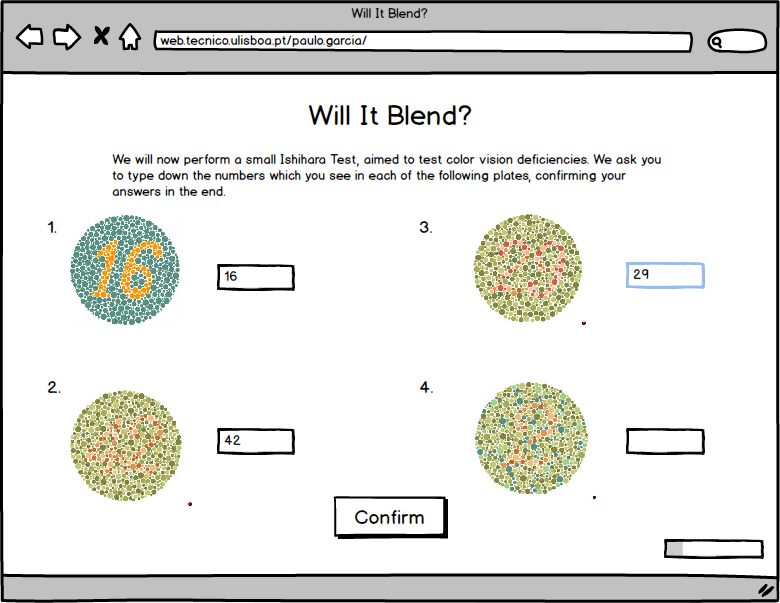
\includegraphics[width=\textwidth]{images/implementation/mockup_ishihara.png}
	  \caption[Mock-up of Color Study's Color Deficiencies Test Phase.]{Mock-up of Color Study's Color Deficiencies Test Phase.}
	  \label{fig:mockup_ishihara}
  \end{minipage} \hfill
	\begin{minipage}{0.49\textwidth}
		\centering
		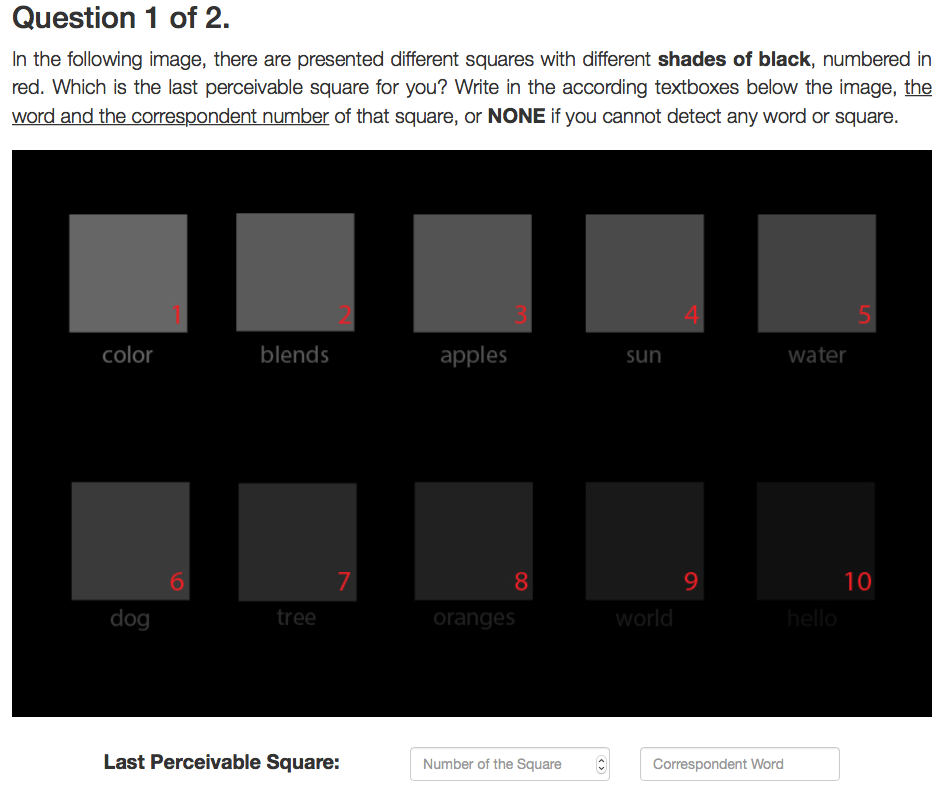
\includegraphics[width=\textwidth]{images/implementation/screen_calibration.png}
		\caption[Screenshot of Color Study's Calibration Testing Phase.]{Screenshot of Color Study's Calibration Testing Phase.}
		\label{fig:screen_ishihara}
	\end{minipage}
\end{figure} \par
%
In this test phase, the users only had to interpret the Ishihara plates and indicate the value which they saw on each of the six plates; these results would be
analyzed later, indicating which users were color vision deficient, therefore leading to a separate analysis. Figures \ref{fig:mockup_ishihara} and
\ref{fig:screen_ishihara} show the evolution between the original mock-up and the implementation of the test phase, once again depicting only a part of the
interface since it is an extensive one.
%
When this phase was finished with success and answers were submitted, the users could proceed to the \textbf{Core Test Phase} of the study, where they would be asked
about the pre-calculated color blendings referred on \ref{sec:impl_designingsolution}.
%
%%%%%%%%%%%%%%%%%%%%%%%%%%%%%%%%% CORE %%%%%%%%%%%%%%%%%%%%%%%%%%%%%%%%%%%%%%%%%%%%%%%%%%%
%
\subsection{Core Test Phase}
\label{subsec:design_core}
%
The last phase is the principal part of the study, which will evaluate the \textbf{Blending of Two Colors}. It was presented the set of color combinations
created from the principal color models' primaries referred before and these color blendings are represent in Table \ref{table:color_blendings}. \par
%
In this test phase, we have composed an interface with the description of the task to fulfill and presented a small set of objects which would be used and
interacted with to provide the colors to the user, and receive his input values. Perhaps, the way color is presented is the most relevant detail: since we
wanted to provide a tool which would be capable of displaying without being influenced by its surrounding of even by the proximity of other colors, the colors
were presented in rounded shapes, accompanied by what we call \emph{\textbf{color sliders}} whenever it was needed input colors from the user. With this,
only the necessary colors are displayed on the circles as the users wish and there is no interference of undesired colors, allowing us to eliminate the
influence of them. The sliders will alternately present a discrete or continuous color scale underneath, according to the type of question which is being
presented to the users. \par
%
\begin{figure}[htbp]
	\centering
  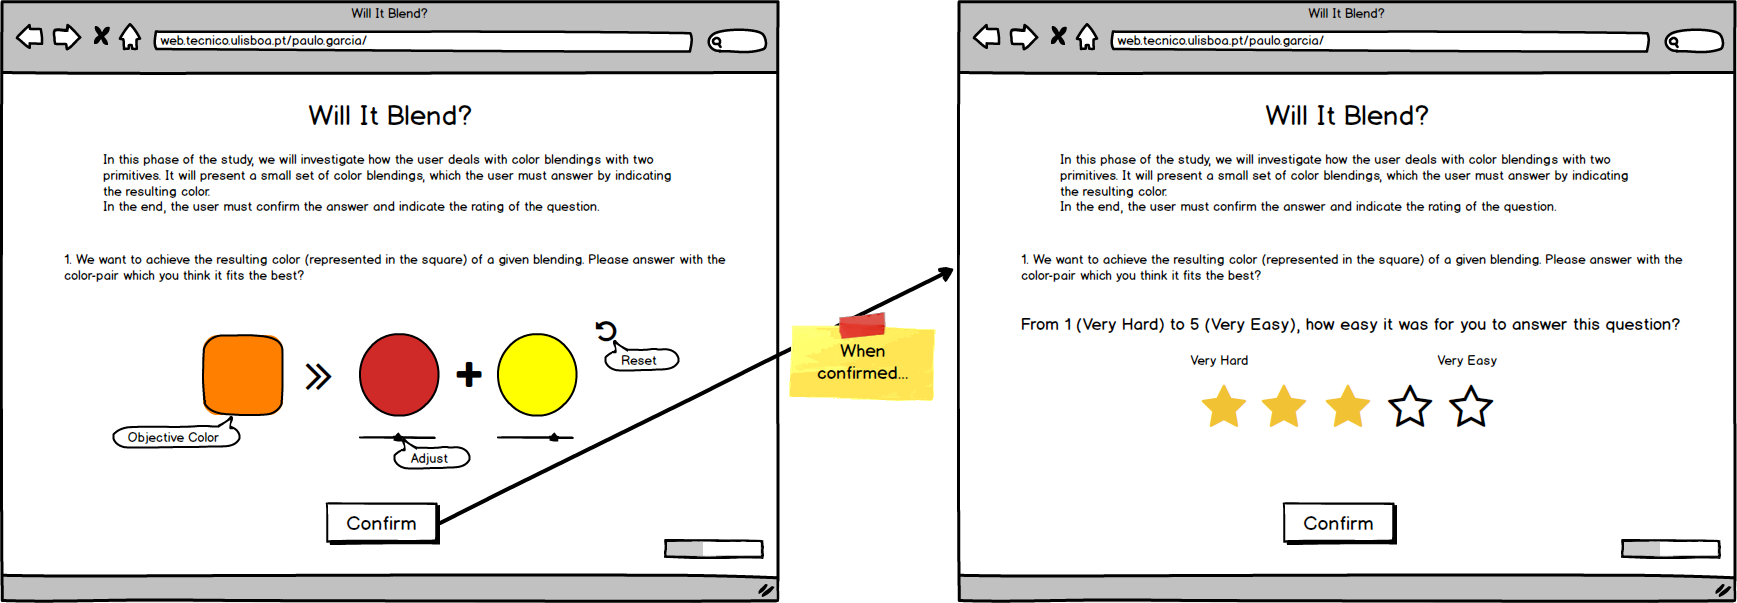
\includegraphics[width=\textwidth]{images/implementation/mockup_core_objTwoColors.png}
  \caption[Mock-up of Color Study's Core Test Phase: present the result and ask the blending-basis.]{Mock-up of Color Study's Core
	Test Phase: presenting the result and asking the blending-basis.}
  \label{fig:mockup_core_1}
\end{figure} \par
%
Since there are two possible types of questions, we have wireframed two screens: \ul{in the first one}, we display a shape filled with the objective color of the
blending and two empty shapes which the users should fill with the colors that they think it corresponds the best to their expectations. These shapes start filled
with an empty color (or white) so the users are not influenced by previously used colors, when answering to another question. There is no particular reason for
the chosen shapes are circles, since \textbf{we are not studying the best visualizations to convey information, when using color blending techniques}. These
shapes presented against a white background so it \textbf{does not influence color perception}, equally spaced between each other, being followed by a small
set of arithmetic operands which \ul{leads the users to realize they have to add a pair of colors}. This screen is depicted in the left side of Figure
\ref{fig:mockup_core_1}. \par
%
\ul{The other screen} presents exactly the same number of circle shapes (three), but one less color slider since this screen is designed to attend questions in
which the blending-basis is already given and the users have to blend them, indicating only \ul{one} answer. These two screens appear, alternately, in a random
fashion so the users do not create any kind of habit or routine when blending the colors from the 32 questions. This screen is depicted in Figure
\ref{fig:mockup_core_2}. \par
%
\begin{figure}[htbp]
	\centering
  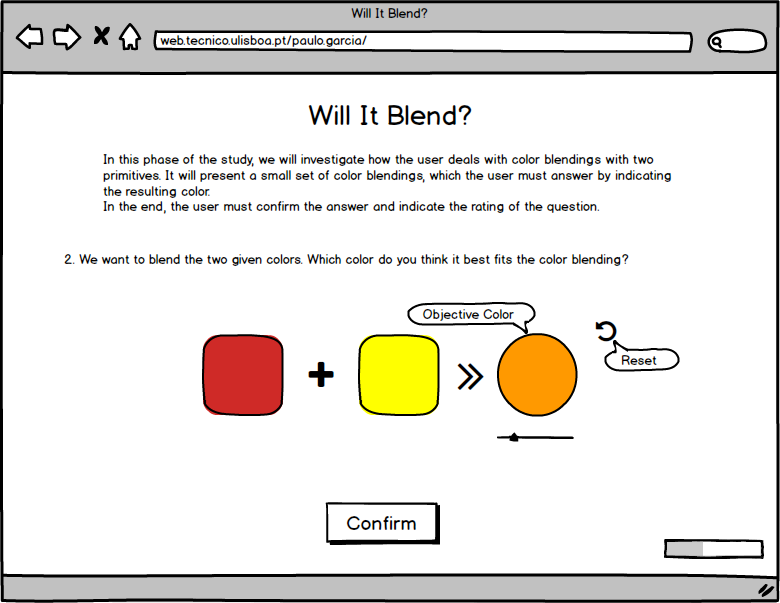
\includegraphics[width=0.4\textwidth]{images/implementation/mockup_core_twoColorsObj.png}
  \caption[Mock-up of Color Study's Core Test Phase: present the blending-basis and ask the result.]{Mock-up of Color Study's Core
	Test Phase: presenting the blending-basis and asking the resulting color.}
  \label{fig:mockup_core_2}
\end{figure} \par
%
The most interesting fact of this test phase is how the color slider works: we chose the HSV Color Model to represent the colors to show, since the
\textbf{HSV Color Model has the best compromise when presenting colors in information visualization} because of its primitives (Hue, Saturation and Value)
which allows to manipulate colors in a better way. However, \textbf{we have chosen to only modify the Hue value and leave the Saturation and Value on its
maximum value}: this way, we could ensure that we could present the entire range of colors at its full saturation and value, also simplifying the gathering
of values from the users. Therefore, the color slider yields a value within the range of $[0º ; 360º]$ degrees which corresponds to an angle in the Hue circle
of the HSV Color Model. \par
%
The color slider has another particularity: the scale of values, though representing continuous angle values, does not presents the values ordered from 0 to 360.
Instead, \textbf{fixed intervals of values are mixed within each other}, so the users do not formulate any mental organization in the moment and do not demonstrate any previous conception or mindset
(\emph{e.g.} the organization of colors according to the color spectrum). The colors were arranged in the following order: \ul{Red-Yellow} ($[0º; 60º]$),
\ul{Blue-Greenish-Blue} ($[240º; 150º]$), \ul{Magenta-Blue} ($[300º; 240º]$), \ul{Greenish-Blue-Yellow} ($[150º; 60º]$) and, lastly, \ul{Magenta-Red} ($[300º; 360º]$). If these
intervals were disposed in its normal order, the order would be seamlessly perceived by the user: this way, \textbf{the users always have to search for the
color they wants to see depicted}. For the questions which the users have to give only one answer (the resulting color from the blend), the color slider
already yields a defined set of pre-calculated colors (the ones present in the referred spreadsheet, on section \ref{sec:impl_designingsolution}), and the
users hand-pick the best-fitting solution from that set. \par
%
However, even the colors represented in the shapes and the ones present in the pre-calculated answers have a particularity, in the laboratory environment: these
pre-calculated values are, with the help of a \emph{Matlab} script, going to be \textbf{converted to adapted color values, according to the .icc color profile
file generated by the Spyder Colorimeter}. This way, we guarantee that no matter if the laboratory environmental conditions change, the colors will always be
presented equally to every user. \textbf{This script processes each possible result for every color pair, in every color model}, converts it to a normalized
CIE-XYZ value and in the end, to an hexadecimal color code to be printed on the shapes of the interface, when time comes for the laboratory user to choose a
color from the color slider. This process was realized before each user session. \par
%
After the users indicated and confirms their answer, \textbf{they were presented a satisfaction question with a 5-point Likert Scale} to double-check the easiness
of each mixture. The question asked was \textbf{"How Easy it was for you to Identify the Mixture?"}; the users had to select the equivalent rating in a
five-star system. If the users were not happy with its response, it was provided a "Reset Mixture" button to clean all parameters. All of these details are
showed in Figure \ref{fig:screen_core}, which shows the resulting interface for the type of questions in which the result was given and the blending-basis
was asked. \par
%
\begin{figure}[htbp]
	\centering
  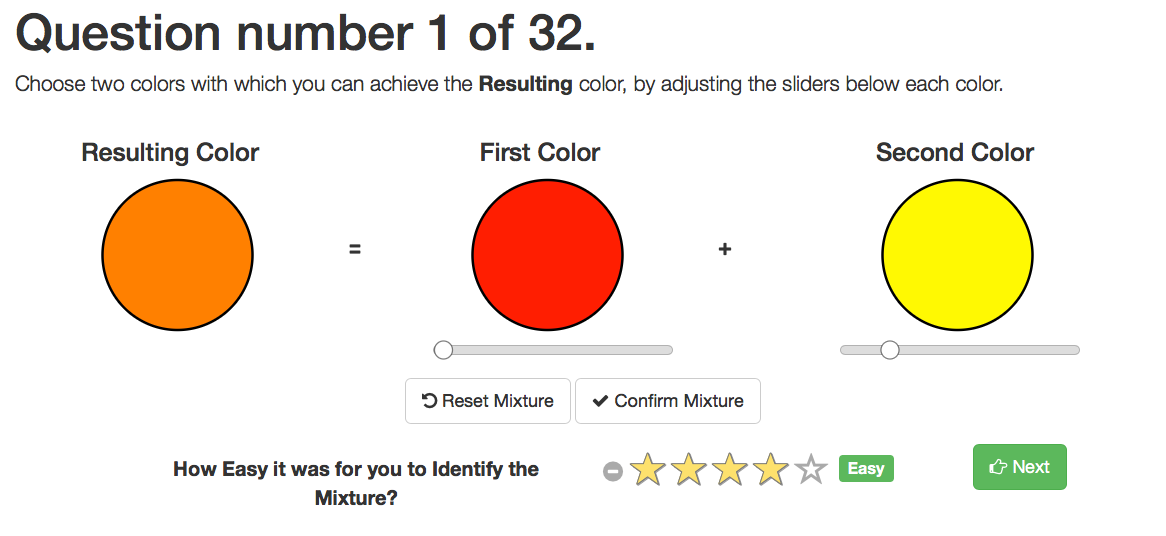
\includegraphics[width=0.8\textwidth]{images/implementation/screen_core.png}
  \caption[Screenshot of Color Study's Core Test Phase: present the result and ask the blending-basis.]{Screenshot of
	Color Study's Core Test Phase: presenting the resulting color and asking the blending-basis.}
  \label{fig:screen_core}
\end{figure} \par
%
In the end, the users were thanked for the time they spent performing the test and it was provided a \ul{Contact Form}, so the users could leave their feedback or
demonstrate the interest (or not) for this subject. All of the data was being stored in the table \emph{results}: a portion of example from the type of data
gathered is present on Table \ref{table:csv_resultsraw}. \par
%
\begin{table}[htbp]
  \resizebox{\textwidth}{!} {
  \begin{tabular} {|c|c|c|c|c|c|c|c|c|c|}
    \hline
    User ID & Type & First Color & Second Color & Third Color & Drags & Time & Rating & Resets & Question ID \\ \hline \hline
    5710cca334d60 & objTwoColors & \#0080FF & hsl(58.69565217391305,1,0.50) & hsl(98.15217391304348,1,0.50) & 992 & 117 & 4 & 2 & 10 \\ \hline
    5745c1c07cc0c & objTwoColors & \#8000FF & hsl(300,1,0.50) & hsl(324.13043478260875,1,0.50) & 645 & 55 & 2 & 1 & 14 \\ \hline
    5745350dc1e22 & objTwoColors & \#0080FF & hsl(226.30434782608697,1,0.50) & NONE & 115 & 11 & 5 & 1 & 10 \\ \hline
    57451c3b38192 & objTwoColors & \#00FF80 & NONE & hsl(150,1,0.50) & 462 & 39 & 5 & 1 & 15 \\ \hline
    574511e99b6d9 & objTwoColors & \#0080FF & hsl(15.652173913043478,1,0.50) & hsl(316.30434782608694,1,0.50) & 442 & 40, & 1 & 1 & 10 \\ \hline
    57427cf6bad0c & twoColorsObj & \#00FFFF & \#FFFF00 & \#46FF9C & 6 & 14 & 3 & 1 & 32 \\ \hline
    5740bda9be3dc & objTwoColors & \#FF7200 & hsl(9.130434782608695,1,0.50) & hsl(50.21739130434783,1,0.50) & 45 & 22 & 5 & 1 & 11 \\ \hline
    573c783748e8b & twoColorsObj & \#00FFFF & \#CBFF00 & \#00FF6B & 44 & 25 & 3 & 1 & 32 \\
    \hline
  \end{tabular}}
  \caption[Excerpt of Raw "Results" Table]{Excerpt of Results Table, with raw data.}
  \label{table:csv_resultsraw}
\end{table} \par
%
\section{Evaluation Criteria}
\label{sec:impl_evaluationcriteria}
%
For a user and its responses to be considered as valid, they have to be evaluated against the following set of rules:
%
\begin{enumerate}
	\item For \ul{Profiling and Ishihara Test Phases}, it is considered as valid the values which are very close from the expected one, since there might
	have been, inadvertently, a slight drift when using the \emph{HTML5} input type "Number" objects.
	\item For \ul{Profiling and Ishihara Test Phases}, it is considered as valid the values which are extremely apart from the expected one, if: \textbf{A:}
	it is an extraordinary situation, for just one plate and no other, and \textbf{B:} if it happens in more than one plate, but in the ones which have a
	presented value, it could be related to an evaluation criteria for that plate.
	\item A user and its answers are considered \textbf{\ul{invalid}} if the results for the majority of plates have extreme values (\emph{e.g.} 1 or 99), and
	the number of answers given is irrelevant.
	\item For Plate \#1, it is considered valid all the users which have answered with the number \textbf{12}, since this is an Instruction/Demonstration plate,
	being interpreted as a control flag, indicating if the user was aware of his task.
\end{enumerate}
%
These criteria will be important in the following section, in which we clean the data gathered along the user color study, process, analyze and infer conclusions.
Besides, these criteria, it should be followed the ones defined in Section \ref{subsec:design_ishihara} which concern the analysis of color vision deficient users.
It will help us defining which users provide useful inputs, and how to separate them among datasets.
